\section{Architektura modelu}
\label{sec:architektura_modelu}

Zastosowany model jest warunkowym modelem dyfuzyjnym przeznaczonym do generowania kodu źródłowego na podstawie opisu zadania (Schemat całej architektury przedstawiliśmy na Rysunku~\ref{fig:model-architecture}). Jego wejście składa się z dwóch części: instrukcji tekstowej określającej wymagane działanie programu oraz częściowo zamaskowanej sekwencji kodu. Model otrzymuje również informację o aktualnym poziomie zaszumienia, czyli o tym, jaka część kodu została ukryta.

Tokeny instrukcji i kodu są najpierw przekształcane na reprezentacje wektorowe. Do każdej reprezentacji dodawana jest informacja o pozycji tokenu w sekwencji, dzięki czemu model może rozróżniać kolejność elementów programu. Reprezentacje instrukcji i kodu są następnie łączone w jedną sekwencję. Tokeny dopełniające, stosowane jedynie w celu wyrównania długości przykładów, są zerowane, aby nie wpływały na dalsze obliczenia.

%\begin{figure}[htbp]
\centering
\setlength{\fboxsep}{8pt}
\fbox{\begin{minipage}{0.88\linewidth}
\centering
\texttt{.env} i zmienne środowiskowe\\
$\downarrow$\\
\texttt{src/train.py::main} $\rightarrow$ \texttt{Config} $\rightarrow$ \texttt{DiffCoderTrainer}\\
$\downarrow$\\
\texttt{data/dataset.csv}\\
$\downarrow$\\
\texttt{ensure\_tokenized\_cache} i \texttt{TokenizedMemmapDataset}\\
$\downarrow$\\
\texttt{MixtureMaskSampler} $\rightarrow$ \texttt{CodeCorruptor}\\
$\downarrow$\\
\texttt{LocalConvDiffCoder.forward}\\
$\downarrow$\\
\texttt{cross entropy} / opcjonalnie \texttt{aligned\_multi\_reference\_cross\_entropy} / opcjonalnie \texttt{CalculateLoss}\\
$\downarrow$\\
\texttt{AdamW} + \texttt{LambdaLR} + \texttt{Trainer}\\
$\downarrow$\\
walidacja, checkpointy, generowanie diagnostyczne
\end{minipage}}
\caption{Aktywna ścieżka treningu zrekonstruowana z \texttt{src/train.py}, \texttt{src/tokenized\_dataset.py}, \texttt{src/diffusion/masking.py} i \texttt{src/diffusion/model.py}.}
\label{fig:architektura}
\end{figure}



\begin{figure}[htbp]
\centering
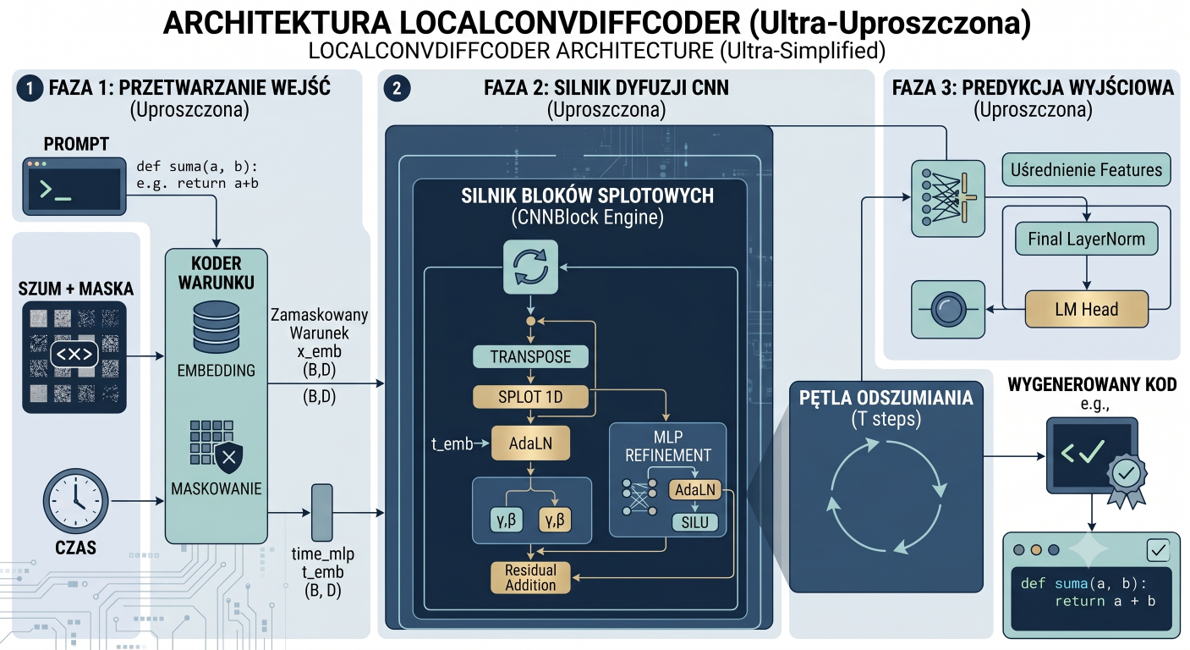
\includegraphics[width=0.9\linewidth]{figures/architecture}
\caption{Schemat architektury modelu dyfuzyjnego z jednowymiarowymi blokami splotowymi.}
\label{fig:model-architecture}
\end{figure}

Główną część modelu stanowi stos bloków splotowych. Sploty jednowymiarowe analizują lokalne zależności między sąsiednimi tokenami, takie jak struktura wyrażeń, argumenty funkcji czy kolejne elementy instrukcji. W kolejnych blokach zwiększane są rozmiar jądra i dylacja, co pozwala obejmować coraz większe fragmenty sekwencji bez konieczności znacznego zwiększania liczby warstw. Dzięki temu model może jednocześnie uwzględniać lokalną składnię oraz zależności występujące między bardziej odległymi częściami programu.

Każdy blok wykorzystuje połączenia rezydualne, normalizację, warstwę nieliniową oraz dropout. Połączenia rezydualne ułatwiają przepływ informacji i stabilizują uczenie głębszej sieci. Normalizacja jest dodatkowo modyfikowana na podstawie poziomu zaszumienia, dzięki czemu sposób przetwarzania sekwencji zależy od liczby ukrytych tokenów. Model może więc inaczej zachowywać się podczas uzupełniania niewielkiego fragmentu kodu, a inaczej podczas odtwarzania prawie całego programu.

Reprezentacje otrzymane w kolejnych blokach są łączone, a następnie wybierana jest część odpowiadająca tokenom kodu. Końcowa warstwa przekształca reprezentację każdej pozycji na rozkład prawdopodobieństwa obejmujący całe słownictwo tokenizatora. Na tej podstawie model przewiduje, jakie tokeny powinny znaleźć się w zamaskowanych miejscach.

Rozmiar reprezentacji, liczba bloków splotowych, poziom dylacji i wartość dropout są parametrami konfiguracyjnymi. Mogą być zatem dostosowywane do wielkości zbioru danych, dostępnych zasobów obliczeniowych oraz wymaganej pojemności modelu.


\section{Uzasadnienie alternatywnej architektury - użycie bloków splotowych zamiast transformera}
\label{sec:uzasadnienie_architektury}

Współczesne systemy generowania kodu są najczęściej oparte na architekturze Transformer oraz mechanizmie uwagi \cite{vaswani2017attention, chen2021evaluating}. Modele te osiągają bardzo dobre wyniki, ponieważ potrafią modelować zależności pomiędzy odległymi fragmentami sekwencji. Jednak ich praktyczne wykorzystanie wiąże się z istotnymi ograniczeniami. Po pierwsze, standardowy mechanizm self-attention ma złożoność obliczeniową rosnącą kwadratowo względem długości sekwencji, czyli $\mathcal{O}(N^2)$. Oznacza to, że przetwarzanie długich plików kodu, zawierających setki lub tysiące tokenów, wymaga bardzo dużej ilości pamięci oraz mocy obliczeniowej. Po drugie, wiele modeli generuje kod autoregresyjnie, czyli token po tokenie od lewej do prawej. Taki sposób generacji powoduje, że błędna decyzja podjęta na wczesnym etapie może zostać utrwalona i wpłynąć na wszystkie kolejne fragmenty wygenerowanego kodu. Problem ten jest trudny do naprawienia bez regeneracji całości, ponieważ model nie wraca do wcześniejszych decyzji.

Problem z pamięcią i złożonością jest szczególnie istotny w przypadku większych projektów programistycznych, gdzie kod nie składa się z pojedynczej, krótkiej funkcji, lecz z wielu zależnych od siebie fragmentów. Model powinien wtedy zachować spójność nazw zmiennych, struktur sterujących, typów danych, importów, definicji funkcji oraz sposobu wykorzystania wcześniej utworzonych elementów programu.

Alternatywą dla klasycznej generacji autoregresyjnej jest maskowana dyfuzja dyskretna, w której model nie musi generować sekwencji wyłącznie od lewej do prawej \cite{austin2021structured, chang2022maskgit}. Zamiast tego proces generacji rozpoczyna się od częściowo zamaskowanej reprezentacji, a następnie model iteracyjnie przewiduje brakujące tokeny. W kolejnych krokach odsłaniane są te fragmenty, co do których model ma największą pewność. Podejście to ma szczególne znaczenie dla kodu: struktura programu często pozwala z dużą pewnością wypełnić niektóre fragmenty — np. zamknięcie bloku, słowo kluczowe \texttt{return}, nawiasy domykające — bez znajomości pozostałych. Pytaniem otwartym pozostaje jednak, jak zaprojektować architekturę modelu, który będzie w stanie efektywnie przewidywać te tokeny przy ograniczonym koszcie obliczeniowym.

W ramach niniejszego projektu proponujemy zbadanie, czy proces maskowanej dyfuzji dyskretnej może zostać zrealizowany nie przy użyciu klasycznego Transformera, lecz za pomocą architektury konwolucyjnej. Główną motywacją tego wyboru jest obserwacja, że kod źródłowy zawiera wiele silnych, lokalnych regularności. Allamanis et al. \cite{allamanis2018survey} pokazują, że kod wykazuje znacznie wyższy stopień powtarzalności niż tekst naturalny — zarówno na poziomie tokenów, jak i krótkich sekwencji. Analiza statystyczna kodu wskazuje, że znaczna część tokenów w typowym pliku źródłowym należy do niewielkiego zbioru wzorców: nawiasów, operatorów, słów kluczowych i krótkich wywołań funkcji \cite{bielik2016phog}. Sugeruje to, że duża część lokalnych decyzń generatywnych nie wymaga dostępu do całego kontekstu sekwencji.

Sieci konwolucyjne są naturalnym kandydatem do modelowania takich zależności, ponieważ analizują dane przez przesuwające się okna o stałym rozmiarze. Dzięki właściwości dzielenia wag, ta sama operacja filtrowania jest stosowana w każdym położeniu sekwencji, co pozwala na wykrywanie powtarzalnych wzorców niezależnie od ich miejsca w pliku. W porównaniu z mechanizmem uwagi, który traktuje każdą parę tokenów symetrycznie, konwolucja może dać lepsze rezultaty w kontekście lokalnym — co w przypadku kodu jest ważne.

Dodatkową zaletą sieci konwolucyjnych jest korzystniejsza skalowalność obliczeniowa. W przeciwieństwie do mechanizmu uwagi, którego koszt rośnie kwadratowo względem długości sekwencji, operacje konwolucyjne mogą być wykonywane z kosztem liniowym względem długości wejścia \cite{wu2019pay, gehring2017convolutional}.

Sama lokalność konwolucji może jednak nie wystarczyć do poprawnego generowania kodu. Programy zawierają bowiem również zależności o większym zasięgu, takie jak użycie zmiennej zdefiniowanej wiele linii wcześniej, odwołania do funkcji, zależności pomiędzy importami a późniejszym kodem czy zgodność typów. Dlatego w projekcie zastosowano architekturę, w której kolejne warstwy konwolucyjne mają wykładniczo rosnące współczynniki rozszerzenia (ang. \textit{dilation rates}), zwiększając efektywne pole recepcyjne modelu geometrycznie wraz z głębokością sieci. Inspiracją dla takiego podejścia są architektury sekwencyjne wykorzystujące rozszerzające się konwolucje, takie jak WaveNet \cite{oord2016wavenet}, oraz prace pokazujące skuteczność modeli konwolucyjnych w zadaniach sekwencyjnych \cite{bai2018empirical}.